
\chapter{向量的坐标运算~~直线与圆}



\section{向量的坐标运算}
\subsection{直角坐标系与向量的坐标}
在初中,我们已学习了平面直角坐标系,其要点如下:
选定一个长度单位,建立两条具有公共原点且互相垂直的数
轴(图5.1),通常一条为水平的数轴,称为横轴或$X$
轴,它的正向是由左到右,另一
条是和它垂直的轴称为纵轴或$Y$
轴,它的正向是从下到上。$X$
轴、$Y$轴总称为坐标轴、坐标轴的交点$O$称为坐标系的原点,这
样我们就说在平面上建立了直角
坐标系$OXY$, 这个平面就叫做
坐标平面,在坐标平面上任取一
点$P$, 过$P$引$X$轴、$Y$轴的垂线,设垂足分别是$M$、$N$, 如
果$M$在$X$轴上的坐标为$x$, $N$在$Y$轴上的坐标为$y$, 那么我
们就说$P$点的坐标是$(x,y)$, 记作$P(x,y)$, $x$称为
横坐标,$y$称为纵坐标。
\begin{figure}[htp]\centering
    \begin{minipage}[t]{0.48\textwidth}
    \centering
\begin{tikzpicture}[>=latex, scale=1]
\draw[->](-1,0)--(4,0)node[right]{$X$};
\draw[->](0,-1)--(0,3)node[right]{$Y$};
\node at (0,0)[below left]{$O$};
\draw[dashed](0,2)node[left]{$N$}--(3,2)node[right]{$P$}--(3,0)node[below]{$M$};
    \end{tikzpicture}
    \caption{}
    \end{minipage}
    \begin{minipage}[t]{0.48\textwidth}
    \centering
    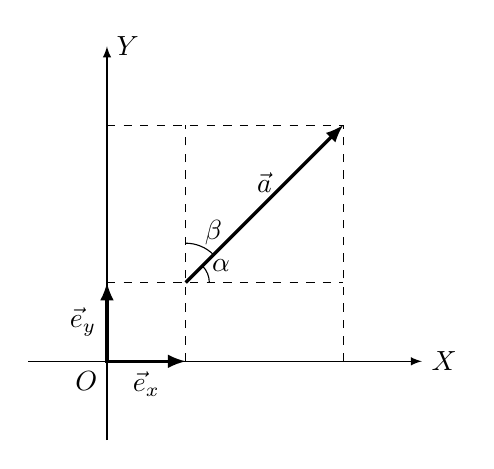
\begin{tikzpicture}[>=latex, scale=1]

\draw[->](-1,0)--(4,0)node[right]{$X$};
\draw[->](0,-1)--(0,4)node[right]{$Y$};
\draw[<->, very thick](0,1)--node[left]{$\vec{e}_y$}(0,0)--node[below]{$\vec{e}_x$}(1,0);
\draw[dashed](0,1)--(3,1);
\draw[dashed](0,3)--(3,3);
\draw[dashed](1,0)--(1,3);
\draw[dashed](3,0)--(3,3);
\draw[->, very thick](1,1)--node[above]{$\vec{a}$}(3,3);
\draw(1.3,1) arc (0:45:.3)node[right]{$\alpha$};
\draw(1,1.5) arc (90:45:.5)node[above ]{$\beta$};
\node at (0,0)[below left]{$O$};

    \end{tikzpicture}
    \caption{}
    \end{minipage}
    \end{figure}


在建立直角坐标系$OXY$的平面上(图5.2),我们
沿$X$轴与$Y$轴的正方向分别取单位向量$\vec{e}_x$、$\vec{e}_y$, 由共面向量
定理可知,对坐标平面上任一向量
$\va$, 存在唯一的有序实数偶$(a_x,a_y)$使
\begin{equation}
    \va =a_x \eX+a_y \eY
\end{equation}
$(a_x,a_y)$就叫做$\va$在直角坐标系
$OXY$上的坐标,记作
\begin{equation}
    \va=(a_x,a_y)
\end{equation}
实质上(5.2)式是(5.1)式的缩写;其中$a_x$叫做$\va$在$X$轴上
的坐标分量,$a_y$叫做$\va$在$Y$轴上的坐标分量。

\begin{blk}
    {定理} 在坐标平面上,如果$\va=(a_x,a_y)$, 则
    \begin{equation}
    \begin{split}
        a_x&=\eX\cdot \va=|\va|\cos\langle\eX,\va\rangle\\
        a_y&=\eY\cdot \va=|\va|\cos\langle\eY,\va\rangle\\
    \end{split}
    \end{equation}
\end{blk}

\begin{proof}
    已知$\va =a_x \eX+a_y \eY$,则
\[\begin{split}
   \eX\cdot \va&=\eX\cdot (a_x\eX+a_y\eY)=a_x\eX\cdot \eX+a_y\eX\cdot \eY\\
   \eY\cdot \va&=\eY\cdot (a_x\eX+a_y\eY)=a_x\eY\cdot \eX+a_y\eY\cdot \eY\\ 
\end{split}\]
由于$\eX,\eY$是单位向量,且$\eX\bot \eY$, 所以,
\[\eX\cdot \eX=\eY\cdot \eY=1,\qquad \eX\cdot \eY=\eY\cdot \eX=0\]
于是得到
\[    \begin{split}
    a_x&=\eX\cdot \va=|\va|\cos\langle\eX,\va\rangle\\
    a_y&=\eY\cdot \va=|\va|\cos\langle\eY,\va\rangle\\
\end{split}\]
\end{proof}

这个定理说的是,\textbf{向量$\va$在$X$轴和$Y$轴上的坐标分量分
别是$\va$在坐标轴上的垂直投影量}。
















































































































































































































\subsection*{习题5.3}
\begin{enumerate}

\item 求通过点$(0,0)$、$(a,0)$、$(0,a)$的圆的方程。
\item 求下列每个圆的圆心和半径。
\begin{enumerate}
    \item $(x-a)(x-b)+(y-c)(y-d)=0$
    \item $(x+y+a)^2+(x-y-a)^2=8a^2$
\end{enumerate}

\item 已知$A(2,-1)$, $B(2,3)$, $C(4,-1)$, 求
$\triangle ABC$的外接圆的圆心和半径。
\item 证明通过$A(a,c)$, $B(b,c)$和$C(b,d)$的圆的方
程是$(x-a)(x-b)+(y-c)(y-d)=0$.
\item $P$是圆心在$A(a,b)$且通过原点的圆上的一动点,求
证$\triangle OAP$重心的轨迹方程是
\[3(x^2+y^2)-4ax-4by+a^2+b^2=0\]
\item 证明$A(6,3)$、$B(5,4)$、$C(1,-2)$和$D(6,
-1)$四点共圆。
\item 一动点到原点的距离的平方是它到定直线$x=1$距离的
4倍,求证这动点的轨迹是点圆$(2,0)$或圆$(x+2)^2
+y^2=8$.
\item 已知三角形由直线$x=2$, $y=4$和$4x+3y=32$围成,
求这三角形内切圆的方程。
\item 已知$A(x_1,y_1)$, $B(x_2,y_2)$, $C(x_3,y_3)$, 一动点
$P(x,y)$使$\overline{AP}^2+\overline{BP}^2+\overline{CP}^2=$常数,证明$P$点的
轨迹是一个圆且它的圆心是$\triangle ABC$的重心。
\item 已知$A(2a,0)$, $C(0,2a)$, $\overline{AC}$是正方形$OABC$的
对角线,一动点$P(x,y)$到这正方形四边距离的平方和
等于$12a^2$, 证明$P$点的轨迹是圆心在$(a,a)$, 半径是$2a$
的圆。
\item 已知$A(3,7)$, $B(-1,5)$, 动点$P(x,y)$使
$\overline{AP}^2+\overline{BP}^2=82$, 证明$P$点的轨迹是半径等于6的圆。
\item 已知$A(3,7)$, $B(1,-1)$, 动点$P$使$\overline{AP}=3\overline{BP}$. 
证明$P$点的轨迹是一个圆且这圆在Y轴上截出的弦长等
于6.
\item 已知$OC$是圆$x^2+y^2-2ax=0$的一条弦,直线$OC$的
斜率是$m$, 求证以$OC$作直径圆的方程是
\[(1+m^2)(x^2+y^2)-2a(x+my)=0\]
\item 如果$a,b$是常数,$\theta$是一动角,求证两直线$x\cos\theta+
y\sin\theta=a$与$x\cos\theta-y\sin\theta=b$的交点的轨迹是一个圆
圆心在原点.半径等于$\sqrt{a^2+b^2}$.
\item 已知一圆与$Y$轴相切于$A(0,-3)$且半径$r=2$, 求
此圆的方程。
\item 已知一圆与两坐标轴相切且通过$A(2,9)$, 求它的方
程。
\item 已知一圆与$X$轴相切于$(5,0)$且在$Y$轴上截出的弦长是10, 求此圆的方程。
\item 求圆:$x^2+y^2=25$与平行线系$x+5y+\lambda=0,\quad (\lambda\in\mathbb{R})$
相交所截弦中点的轨迹。
\item 求二圆$x^2-12x+y^2-10y+52=0$, $x^2+18x+y^2+
20y+60=0$的圆心距及原点到连心线的距离。
\item 在直线系$y-7+\lambda(x+1)=0$中,求与圆$x^2+y^2=2$
相切之直线。
\item 求通过点$(5,-2)$且与已知直线$3x-y-1=0$相切于
点$(1,2)$的圆的方程。
\end{enumerate}

\section*{复习题五}
\begin{enumerate}
    \item 一个正六边形边长是$a$, 中心在坐标原点,两个顶点在
    $X$轴上,求各顶点的坐标。
    \item 以原点为起点的三个力$\vec{F}_1=(9,7)$, $\vec{F}_2=(-6,4)$, 
    $\vec{F}_3=(1,2)$; 求它们的合力坐标和方向。
    \item 已知一个三角形三边中点的坐标分别是$(x_1,y_1)$, $(x_2,
    y_2)$, $(x_3,y_3)$, 求三个顶点的坐标。
    \item 已知$A(-1,3)$, $B(4,1)$, 直线$AB$与$X$轴,$Y$轴
    分别相交于$C$、$D$两点,求$C$、$D$两点分割$AB$的比
    值。
    \item 已知$P(x,y)$, $A(x_1,y_1)$, $B(x_2,y_2)$且
    \[x=x_1+t(x_2-xy),\qquad y=y_1+t(y_2-y_1)\]
    求证:$P$点按定比$\mu=\frac{t}{1-t}$
    分割$\Vec{AB}$.
    \item 已知直线$\ell:\; ax+by+c=0$及$P_1(x_1,y_1)$, $P_2(x_2,  y_2)$两点,
    求证直线$\ell$与直线$P_1P_2$的交点把$\Vec{P_1P_2}$按定比
$-\frac{ax_1+by_1+c}{ax_2+by_2+c}$分割。
\item 用坐标法证明:直角三角形斜边的中点到三顶点的距离
相等。
\item 用坐标法证明勾股定理的逆定理。
\item 已知:四边形一组对边的平方和等于另一组对边的平方
和,用坐标法证明:两条对角线互相垂直。
\item 已知$G$是$\triangle P_1P_2P_3$的重心,用坐标法证明:
\[S_{GP_2P_3}=\frac{1}{3}S_{P_1P_2P_3}\]
\item 已知$A(1,2)$、$B(8,4)$、$C(4,10)$, 求一点
使$\triangle PAB$、$\triangle PBC$、$\triangle PCA$的面积相等,并解释
这个结果的几何意义。
\item 一条直线经过点$P(1,-1)$, 它的倾角等于直线
$y=x$倾角的3倍,求这条直线的方程。
\item 已知$A(-3,2)$, $B(-2,-2)$, $C(4,0)$.求:
\begin{enumerate}
    \item $\triangle ABC$ $\overline{BC}$边上的中线方程;
    \item $\overline{AC}$边上的高线方程,并求出这条高的长。
\end{enumerate}

\item 一条直线经过$(2,4)$并且和直线$x+y-4=0$的夹角
是$\pi/4$,
求这条直线的方程。
\item 一条光线从$P_0(6,4)$射出和$X$轴正向交成锐角$\alpha$, 
遇到$X$轴反射,已知$\tan\alpha=2$, 求入射光线和反射光线
所在的直线方程。
\item 从原点向直线$3x-2y+7=0$作垂线,求垂线段的长和
垂足的坐标。
\item 在直线$2x-3y=0$上求一点,使这点和原点之间的距
离等于这点到直线$2x+3y-2=0$之间的距离。
\item 已知点$P(3,2)$, 直线$\ell:\; y=4x+3$, 求$P$点到直
线$\ell$的距离,垂线足的坐标,点$P$关于$\ell$的轴对称点的
坐标。
\item 已知直线$ax+by+c=0$和点$P_0(x_0,y_0)$, 求$P_0$点关
于直线$ax+by+c=0$的轴对称点的坐标。
\item 已知$\ell_1:\; 3x-4y-17=0$, $\ell_2:\; y=4$, $\ell_3:\; 12x+5y-12=0$, 求证点$(-4,-1)$是$\ell_1,\ell_2,\ell_3$两两相交
所构成三角形的内心。
\item 求直线$3x-4y+6=0$与$12x-5y-9=0$交角平分
线的方程。
\item 证明通过点$(a,b)$的直线方程可写为
\[\lambda_1(x-a)+\lambda_2(y-b)=0\]
\item 设$P_1(x_1,y_1)$及$P_2(x_2,y_2)$为两定点,过$P_1$作直线
交$Y$轴于$B$点,过$P_2$作直线与过$P_1$之直线垂直,交$X$
轴于点$A$, 求$AB$中点的轨迹。
\item 求下列各圆的方程。
\begin{enumerate}
 \item 过$O(0,0)$, $A(-5,0)$, $B(0,3)$;
\item 中心在$C(-3,4)$与$3x+8y-6=0$相切;
\item 过$A(4,3)$, $(-2,5)$, 圆心在$2x-3y=0$上;
\item 过$A(5,-2)$与直线$3x-y-1=0$相切于点$(1,
2)$;
\item 通过$O(0,0)$, 圆心在$x=2$上且与直线$x+
y-8=0$相切。
\end{enumerate}

\item 求两圆$x^2+y^2-x+2y=0$, $x^2+y^2+2x-y=9$的
交点的坐标。
\item 求两圆$x^2+y^2+ax+by=0$, $x^2+y^2+bx-ay=0$
的交点的坐标。
\item 求两圆$x^2+y^2=10$, $x^2+y^2-10x-10y+30=0$公
共弦所在直线的方程。
\item 已知圆$x^2+y^2-4x-5=0$和点$A(5,4)$, 求圆心
在$A$点且与已知圆外切的圆的方程。
\item 已知二圆$x^2+y^2-6x+8y=0$, $x^2+y^2+2x-12y
+1=0$, 求通过二圆圆心的直线方程。
\item 求两圆$(x-a_1)^2+(y-b_1)^2=r^2_1$, $(x-a_2)^2+(y-
b_2)^2=r^2_2$正交(即在两圆公共点处的切线互相垂直)
的条件是
\[(a_1-a_2)^2+(b_1-b_2)^2=r_1^2+r_2^2\]
\item 一条$AB=2a$的两个端点$A$和$B$分别在$X$轴和$Y$轴上滑
动,求$\overline{AB}$中点$M$的轨迹。
\item 已知$A(2,2)$, $\triangle OAC$是等边三角形,且$O$、$A$、
$C$构成反时针排列,求点$C$的坐标。
\item 已知$A(x_1,y_1)$, $B(x_2,y_2)$, $C(x_3,y_3)$, 求证
$\triangle ABC$的重心到三顶点的距离平方和为最小。
\item 已知$A(-5,4)$, 过点$A$作条直线使它与两坐标轴
相交所成的三角形的面积等于5个平方单位,求证这条
直线的方程是$8x+5y+20=0$或$2x+5y-10=0$.
\item 已知点$A(a,b)$在第I象限,过点$A$求一条直线使与坐
标轴交成的三角形面积最小,并求出最小面积的值。

\item 如果
\begin{multicols}{2}
    \begin{enumerate}
        \item $D=0$
        \item $E=0$
        \item $F=0$
        \item $D=0$, $E=0$
        \item $D=0$, $F=0$
        \item $E=0$, $F=0$
    \end{enumerate}
\end{multicols}
那么圆$x^2+y^2+2Dx+2Ey+F=0$对
坐标系的位置有什么特征。
\item 已知$P_0(x_0,y_0)$是圆:$x^2+y^2+2Dx+2Ey+F=0$
外任意一点,若自$P_0$向圆引切线$P_0T$, $T$为切点,求
证:$\overline{P_0T}^2=x_0^2+y_0^2+2Dx_0+2Ey_0+F$.
\item 为了使圆$x^2+y^2+2Dx+2Ey+F=0$
\begin{enumerate}
\item 不与$X$轴相交;    
\item 和$X$轴交于两点;    
\item 和$X$相切,
\end{enumerate}
问它的方程中的系数分别应该满足怎样的条件?

\item 求圆心在点$(4,0)$并与直线$3x-4y+1=0$相切的
圆的方程。
\item 已知$\odot C$的圆心$C$在直线$x-y-4=0$上,并经过两圆
$C_1:\; x^2+y^2-4x-3=0$和$C_2:\; x^2+y^2-4y-3
=0$的交点,求$\odot C$的方程。
\item 一动点到已知正方形的各顶点的距离平方和是一个常
数,求这动点的轨迹方程,并说明轨迹是什么图形。
\item 已知点$Q(4,0)$, 点$P(x,y)$是圆:$x^2+y^2=4$上一
动点,求$PQ$中点的轨迹方程。
\item 当$\lambda$为何值时,直线$\lambda x-y-\lambda-1=0$与圆$x^2+y^2-
4x-2y+1=0$相交,相切或相离。
\end{enumerate}